\documentclass[tikz,margin=2mm]{standalone}
\usepackage{tikz}
\usetikzlibrary{arrows.meta,calc}

\begin{document}
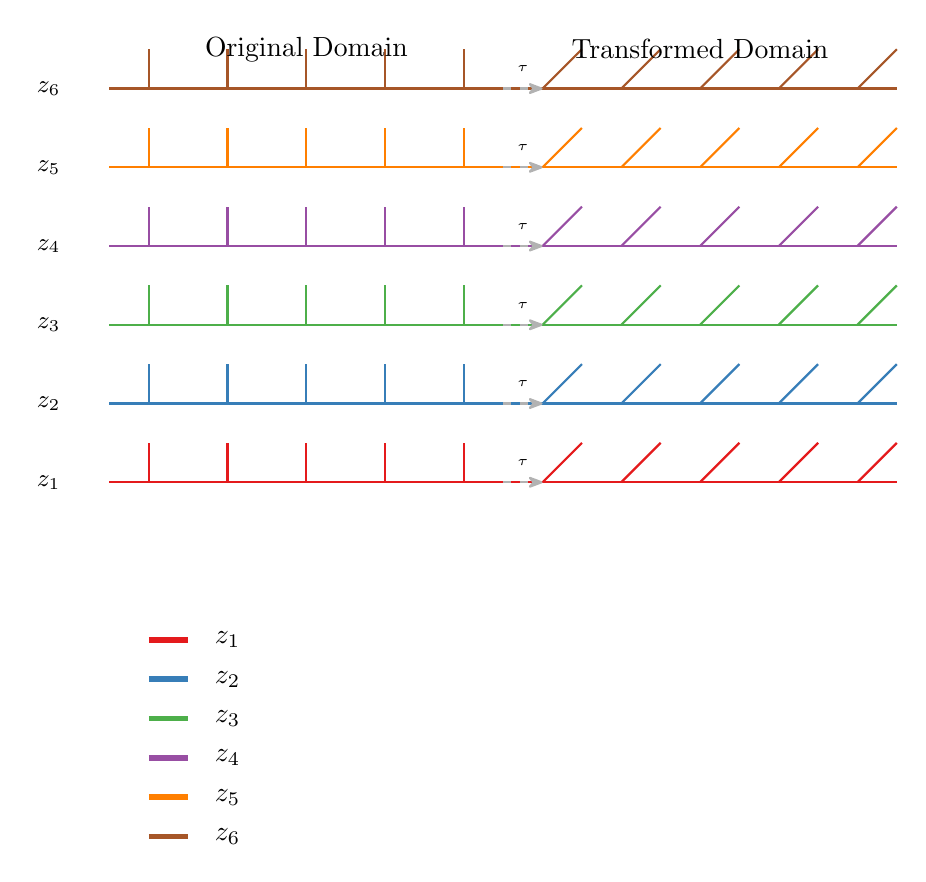
\begin{tikzpicture}[
    >={Stealth[round]},
    row/.style={thick, color=#1},
    spectral/.style={anchor=east, font=\small},
    transform/.style={->, thick, dashed, color=gray!60}
]

% Define colors for rows
\definecolor{row1}{RGB}{228,26,28}
\definecolor{row2}{RGB}{55,126,184}
\definecolor{row3}{RGB}{77,175,74}
\definecolor{row4}{RGB}{152,78,163}
\definecolor{row5}{RGB}{255,127,0}
\definecolor{row6}{RGB}{166,86,40}

% Original domain grid
\foreach \i in {1,...,6} {
    % Spectral parameters
    \node[spectral] at (-1,\i) {$z_{\i}$};
    
    % Horizontal rows
    \draw[row=row\i] (-0.5,\i) -- (4.5,\i);
    
    % Vertical lines
    \foreach \j in {0,...,4} {
        \draw[row=row\i] (\j,\i) -- (\j,\i+0.5);
    }
}

% Transformed domain overlay
\begin{scope}[xshift=5cm]
    \foreach \i in {1,...,6} {
        % Shifted horizontal rows
        \draw[row=row\i] (-0.5,\i) -- (4.5,\i);
        
        % Transformed vertical connections
        \foreach \j in {0,...,4} {
            \draw[row=row\i] (\j,\i) -- (\j+0.5,\i+0.5);
        }
    }
\end{scope}

% Transformation arrows
\foreach \i in {1,...,6} {
    \draw[transform] (4.5,\i) -- (5,\i);
    \node at (4.75,\i+0.25) {\tiny $\tau$};
}

% Domain labels
\node at (2,6.5) {Original Domain};
\node at (7,6.5) {Transformed Domain};

% Color legend
\foreach \i/\col in {1/row1,2/row2,3/row3,4/row4,5/row5,6/row6} {
    \draw[\col, line width=2pt] (0,-0.5-\i/2) -- (0.5,-0.5-\i/2);
    \node at (1,-0.5-\i/2) {$z_{\i}$};
}

\end{tikzpicture}
\end{document}